\section{Tamamlayıcı vaka: aynı satır, aynı kişi midir?}
\label{sec:v3-eslesme}

\textbf{Soru ve sınır.} İki sütunu çıkarmadan önce gerçekten aynı
öğrencinin ölçümlerini eşleştirdiğimizi nasıl denetleriz? Bu vaka,
B11'deki testi yeniden öğretmek yerine eşleşmenin kurulmasını ve
ölçümlerin anlamını inceler. UCI matematik dosyasında G1 ilk dönem,
G3 yıl sonu notudur; ikisi de 0--20 ölçeğindedir
\citep{cortez2008data}. Aynı sayısal ölçek, eşdeğer sınav tekrarını
veya rastgele atanmış bir müdahalenin ön--son ölçümünü kanıtlamaz.

\textbf{Kayıt anahtarının kökeni.} B11'in \texttt{id} sütunu, kaynak
dosyanın sırasından üretilmiş yerel anahtardır; özgün öğrenci kimliği
değildir. Bu vakada önce kaynakla eşleştirilip sabitlenir, sonra G1 ve
G3 tabloları ayrılır. G3 tablosu bilerek ters sırada saklanır; anahtarlar
değişmez. İki tabloya sonradan ayrı ayrı yeni sıra numarası vermek,
eşleşmeyi korumaz. Bu anahtar matematik ve Portekizce dosyalarını
birleştirmek için de kullanılamaz.

\textbf{Veri kabulü.} Yerel B11 kopyasının G1/G3 değerleri kaynak
matematik dosyasının 395 satırıyla karşılaştırıldı. Ayrı tablolardaki
anahtarlar boş değildir ve her birinde benzersizdir. Anahtar kümeleri
aynıdır; 395 anahtar eşleşmesi ve 395 tam çift vardır. Sıfır G3 notlu
38 kayıt eksik sayılmadı. Ana veri değiştirilmedi; bu kayıtlar yeni
ve bağımsız bir araştırma oluşturmaz.

\begin{mistakebox}
\textbf{Aynı ortalama, doğru eşleşme demek değildir.} G3 tablosunun
ters çevrilmiş sırasını anahtarı dikkate almadan G1 ile yan yana
koyarsak 394 kayıt başka bir öğrencinin notuyla eşleşir; ortadaki
tek anahtar yerinde kalır. Bu, yalnız hata göstermek için yapılan
bir denemedir; geçerli öğrenci içi değişim analizi değildir.

Bütün değerler birer kez kullanıldığında herhangi bir sıra değişimi
$\pi$ için
\[
\frac{1}{n}\sum_i\bigl(G3_{\pi(i)}-G1_i\bigr)
=\overline{G3}-\overline{G1}
\]
olur. Bu koşullarda ortalama fark aynıdır; buna rağmen eşleşmeler
ve farkların yayılımı değişebilir. Yalnız ortalamaların
aynılığını kontrol etmek bu hatayı yakalayamaz.
\end{mistakebox}

\begin{table}[H]
\centering
\caption{V3'te doğru eşleşme ile yapay sıra hatasının karşılaştırılması}
\label{tab:v3-sira-hatasi}
\begin{tabular}{@{}lrr@{}}
\toprule
İşlem & Ortalama fark & Farkların SS'si \\
\midrule
Anahtarla doğru eşleşme & $-0{,}493671$ & 2,762482 \\
Yapay, hatalı sıra eşleştirmesi & $-0{,}493671$ & 5,337049 \\
\bottomrule
\end{tabular}
\end{table}
Hatalı satırın standart sapması, gerçek öğrenci içi farkların standart
sapması olarak kullanılamaz. Bu hatalı çiftlerden yeni bir test veya
güven aralığı raporlanmamıştır. B11'in geçerli eşleştirilmiş sonuçları
Tablo~\ref{tab:b11-dogrulanmis-test} içindedir.

\textbf{İki ayrı kontrol kapısı.} Önce kayıt anahtarlarının kökenini
doğrulayın; ardından benzersizlik, eşleşmeyen anahtar ve ölçüm
eksikliği kontrollerini yapın. Benzersiz fakat yanlış atanmış anahtarlar
teknik birleştirme denetiminden geçebilir. Bire bir eşleşme, kaynak
eşleştirmesinin ve ölçüm protokolünün yerine geçmez.

\par\noindent\begin{minipage}{\linewidth}
\textbf{Python: satır sırası yerine anahtar.} Paket kökünden bloğun
tamamını çalıştırın. \texttt{outer} eşleşmeyen kayıtları görünür
tutar; \texttt{validate} çoğul anahtarları engeller. Kontrol başarısızsa
silerek, doldurarak veya ilk kaydı seçerek devam etmeyin.

\begin{lstlisting}[style=prismPythonApp]
import pandas as pd

kok = "companion/vakalar/v3-eslesme/"
ilk = pd.read_csv(kok + "g1.csv")
son = pd.read_csv(kok + "g3-reversed.csv")
assert ilk.id.notna().all() and son.id.notna().all()
assert ilk.id.is_unique and son.id.is_unique
cift = ilk.merge(son, on="id", how="outer",
    validate="one_to_one", indicator=True, sort=True)
print(cift["_merge"].value_counts())
assert cift["_merge"].eq("both").all()
assert cift[["g1", "g3"]].notna().all().all()
assert cift.g1.between(0, 20).all()
assert cift.g3.between(0, 20).all()
assert len(cift) == 395
fark = cift.g3 - cift.g1
print("Tam cift:", len(fark))
print("Ortalama:", fark.mean(), "SS:", fark.std(ddof=1))
print("Negatif / sifir / pozitif:",
      (fark < 0).sum(), (fark == 0).sum(), (fark > 0).sum())
\end{lstlisting}
\end{minipage}\par

\textbf{Eksik eş ile eksik ölçüm farklıdır.} Ayrı, açıkça yapay
denemelerde G3 tablosundan bir satır kaldırıldığında 394 anahtar
eşleşmesi ve bir karşılıksız G1 kaydı bulunur. Satır korunup yalnız
notu boş bırakıldığında ise 395 anahtar eşleşmesi, fakat 394 tam çift
vardır. Bir anahtar yinelendiğinde bire bir birleştirme reddedilir;
yalnız G3'te bulunan ek anahtar da raporlanır. Bu denemeler gerçek
dosyadaki eksiklikler değildir; kaynak üzerinde silme veya doldurma
yapılmamıştır. Denetleyici, uygunsuz örnekte analiz üretmeden durur.

\begin{figure}[H]
\centering
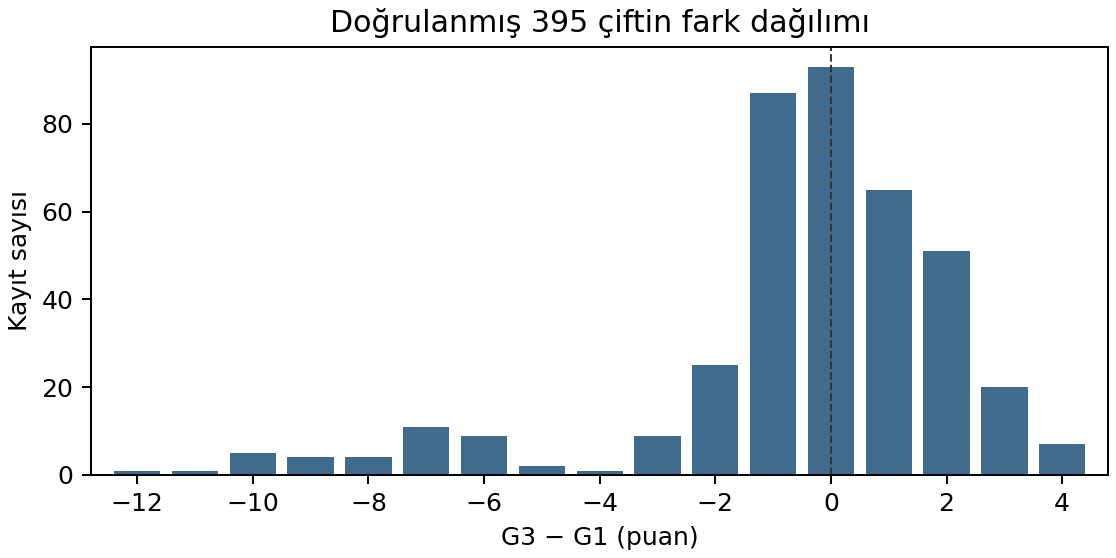
\includegraphics[width=\linewidth]{companion/vakalar/v3-eslesme/differences.png}
\caption{V3'te doğrulanmış G3--G1 farklarının sayımları. Sıfır G3
notları korunmuştur; yapay hatalı eşleşmeler grafiğe dahil değildir.}
\label{fig:v3-farklar}
\end{figure}

\textbf{Farkların anlamı.} Doğru eşleşmede 159 fark negatif, 93 fark
sıfır, 143 fark pozitiftir. Medyan 0; en küçük fark $-12$, en büyük
fark 4 puandır. Ortalama farkın negatif olması her öğrencinin notunun
düştüğü anlamına gelmez. Grafik, kimin öğretimden ne kadar yararlandığını
veya farklı öğrencilerin bağımsızlığını kanıtlamaz. Dönem notlarının
nasıl oluşturulduğu açıklanmadan farkı yalnız öğrenme kaybı diye
adlandırmayız.

\textbf{Ham çift ile özet girdi.} Küçük B14 paketindeki 24 çift,
ortalama fark $-3{,}2$ ve fark standart sapması 6 bilgisi başka bir
öğretim örneğidir; bu 395 kaydın özeti değildir. O üç özetten standart
hata ve test hesabı yapılabilir; hangi kişinin eksik eşinin bulunduğu,
anahtarların yinelenmesi veya fark grafiği geri kurulamaz. Aynı özeti
veren farklı ham veriler olabilir; 24 çifti bu veriden türetmeyiz.

\subsection{Görevler, kontrol yanıtları ve puanlama}
Her görevin iki bileşeni vardır. Bileşen başına doğru, gerekçeli yanıt
1 puan; eksik veya yanlış yanıt 0 puandır. Toplam 10 puan.

\begin{enumerate}
\item \textbf{Anahtar ve birim.} \texttt{id}'nin kökenini açıklayın;
ayrı sıralanmış iki tabloyu yeniden numaralandırmak yerine doğru
eşleşmeyi nasıl koruyacağınızı yazın.
\item \textbf{Yanlış eşleşmeyi yakalama.} Tablodaki iki ortalama
neden aynıdır? Buna rağmen ikinci satır neden geçerli değişim
analizi değildir?
\item \textbf{İki tür eksiklik.} Bir satırın yokluğu ile notun
boşluğu için anahtar eşleşmesi/tam çift sayısını ayrı yazın. Yinelenen
anahtarda neden otomatik olarak ilk kayıt alınmamalıdır?
\item \textbf{Dağılım ve yorum.} Negatif ortalamayı herkesin notunun
düşmesi şeklinde yorumlayan cümleyi sayımlarla düzeltin; ardından
bu farkın neden tek başına öğretimin nedensel etkisi olmadığını açıklayın.
\item \textbf{Özetin sınırı.} Küçük B14'ün 24 çiftlik özetinden
bir hesaplanabilir nicelik ve bir denetlenemeyecek kayıt özelliği
verin. Bu özeti mevcut 395 çiftle birleştirmemenizin nedenini belirtin.
\end{enumerate}

\textbf{Gerekçeli kontrol yanıtları.}
\begin{enumerate}
\item Yerel anahtar kaynak satırına bağlıdır; özgün kişi kimliği değildir
(1). Bölmeden önce korunur, kaynakla denetlenir ve tablolar bu sabit
anahtarla birleştirilir; yeniden sıra numarası üretilmez (1).
\item Her sütunun toplamı değişmediğinden ortalama fark korunur (1).
394 yanlış ortak nedeniyle farklar artık aynı öğrencinin iki notu
değildir; standart sapmanın da değişmesi hatayı görünür kılar (1).
\item Satır yoksa 394/394, yalnız not eksikse 395/394 bulunur (1).
Yinelenme kaynak kayıtlarına dönülerek çözülmelidir; ilk satırı seçmek
ölçüm veya anahtar hatasını gizleyebilir (1).
\item 159 negatif yanında 93 sıfır ve 143 pozitif fark bulunduğundan
``herkesin notu düştü'' yanlıştır (1). Eşdeğer ölçüm ve rastgele
müdahale ataması bu kayıtlardan doğrulanmaz; puan farkı tek başına
öğretim etkisi değildir (1).
\item Standart hata $6/\sqrt{24}$ hesaplanabilir, fakat ham
anahtar/eş eksikliği denetlenemez (1). Bunlar farklı öğretim örnekleridir;
24 çift bu 395 gözlemin alt grubu veya bağımsız tekrarı sayılamaz (1).
\end{enumerate}

\textbf{Kısa rapor örneği.} ``Kaynak satırıyla eşleştirilen sabit
yerel anahtarlar üzerinden 395 tam çift doğrulanmış; sıfır yıl sonu
notları korunmuştur. G3 eksi G1 ortalama farkı $-0{,}494$ puan,
medyanı 0'dır; 159 negatif, 93 sıfır ve 143 pozitif fark vardır.
Bu betimleme eşdeğer sınavlardan elde edilen öğrenme kaybı veya
bir öğretim müdahalesinin nedensel etkisi olarak sunulmamıştır.''

Python aktarımı ve ayrı anahtar sözlüğüyle hesap kontrol edilmiştir;
yeni R/SPSS çalıştırması veya bağımsız saha kimliği doğrulaması
yapılmamıştır. Kod, sözlük, hata denemeleri ve dosya özetleri
\nolinkurl{companion/vakalar/v3-eslesme/} klasöründedir.